\documentclass[border=4pt]{standalone}
\usepackage{tikz}
\usepackage{pgfplots}
\pgfplotsset{compat=1.18}
\usepackage{booktabs}
\usepackage{array}
\usepackage{colortbl}
\usepackage{amsmath,amssymb}
\usetikzlibrary{positioning, arrows.meta, shapes.geometric, calc, fit, backgrounds}

\definecolor{oursblue}{RGB}{31,78,121}
\definecolor{tradgray}{RGB}{130,145,150}
\definecolor{oursaccent}{RGB}{192,57,43}

\begin{document}
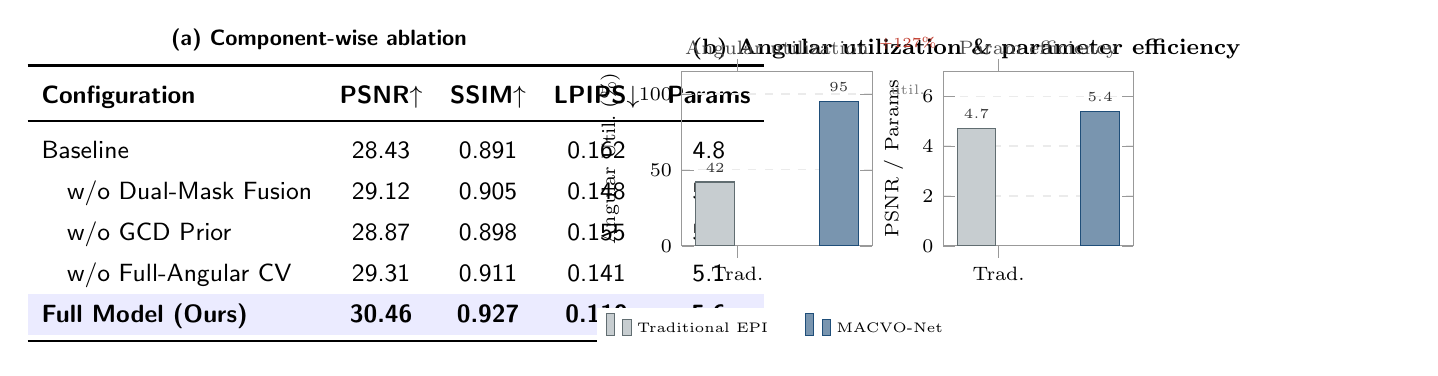
\begin{tikzpicture}[font=\sffamily]

% ========== Panel (a): Ablation Table ==========
\node[anchor=north west, inner sep=0pt] (panelA) at (0,0) {%
\begin{minipage}{7.4cm}
\centering
{\footnotesize\bfseries (a) Component-wise ablation}\\[4pt]
\renewcommand{\arraystretch}{1.35}%
\setlength{\tabcolsep}{5pt}%
\small
\begin{tabular}{lcccc}
\toprule
\textbf{Configuration} & \textbf{PSNR}$\uparrow$ & \textbf{SSIM}$\uparrow$ & \textbf{LPIPS}$\downarrow$ & \textbf{Params} \\
\midrule
Baseline                          & 28.43 & 0.891 & 0.162 & 4.8 \\
\quad w/o Dual-Mask Fusion        & 29.12 & 0.905 & 0.148 & 5.2 \\
\quad w/o GCD Prior               & 28.87 & 0.898 & 0.155 & 5.4 \\
\quad w/o Full-Angular CV         & 29.31 & 0.911 & 0.141 & 5.1 \\
\rowcolor{blue!8}
\textbf{Full Model (Ours)}        & \textbf{30.46} & \textbf{0.927} & \textbf{0.119} & \textbf{5.6} \\
\bottomrule
\end{tabular}
\end{minipage}%
};

% ========== Panel (b): Bar Charts ==========
\coordinate (bStart) at ($(panelA.north east)+(0.9cm,0)$);

% Panel b title
\node[anchor=north west, font=\footnotesize\bfseries, text width=9cm] at (bStart)
  {(b) Angular utilization \& parameter efficiency};

% Bar chart 1: Angular Utilization Rate
\begin{axis}[
    name=chart1,
    at={($(bStart)+(0,-0.55cm)$)},
    anchor=north west,
    width=4cm, height=3.8cm,
    ybar,
    bar width=14pt,
    symbolic x coords={Trad., Ours},
    xtick=data,
    ymin=0, ymax=115,
    ylabel={Angular Util.\ (\%)},
    ylabel style={font=\scriptsize},
    xticklabel style={font=\scriptsize},
    yticklabel style={font=\scriptsize},
    title={Angular utilization},
    title style={font=\scriptsize, yshift=-5pt, text=black!70},
    nodes near coords,
    nodes near coords style={font=\tiny, text=black!80, anchor=south},
    enlarge x limits=0.7,
    axis line style={black!40},
    tick style={black!40},
    ymajorgrids=true,
    grid style={black!8, dashed},
    legend style={at={(0.5,-0.35)},anchor=north,legend columns=2,font=\tiny,draw=none,/tikz/every even column/.append style={column sep=0.4cm}},
]
\addplot[fill=tradgray!45, draw=tradgray!75!black] coordinates {(Trad.,42)};
\addplot[fill=oursblue!60, draw=oursblue] coordinates {(Ours,95)};
\legend{Traditional EPI, MACVO-Net}
\end{axis}

% Bar chart 2: Parameter Efficiency
\begin{axis}[
    name=chart2,
    at={($(chart1.north east)+(0.9cm,0)$)},
    anchor=north west,
    width=4cm, height=3.8cm,
    ybar,
    bar width=14pt,
    symbolic x coords={Trad., Ours},
    xtick=data,
    ymin=0, ymax=7,
    ylabel={PSNR / Params},
    ylabel style={font=\scriptsize},
    xticklabel style={font=\scriptsize},
    yticklabel style={font=\scriptsize},
    title={Param efficiency},
    title style={font=\scriptsize, yshift=-5pt, text=black!70},
    nodes near coords,
    nodes near coords style={font=\tiny, text=black!80, anchor=south},
    enlarge x limits=0.7,
    axis line style={black!40},
    tick style={black!40},
    ymajorgrids=true,
    grid style={black!8, dashed},
]
\addplot[fill=tradgray!45, draw=tradgray!75!black] coordinates {(Trad.,4.7)};
\addplot[fill=oursblue!60, draw=oursblue] coordinates {(Ours,5.4)};
\end{axis}

% Improvement annotation between charts
\node[font=\tiny\bfseries, text=oursaccent, anchor=south] 
  at ($(chart1.north east)!0.5!(chart2.north west)+(0,0.15cm)$) {$+127\%$};
\node[font=\tiny, text=black!50, anchor=north] 
  at ($(chart1.north east)!0.5!(chart2.north west)+(0,-0.05cm)$) {util.};

\end{tikzpicture}
\end{document}